% Options for packages loaded elsewhere
\PassOptionsToPackage{unicode}{hyperref}
\PassOptionsToPackage{hyphens}{url}
%
\documentclass[
]{article}
\title{Lab 1}
\author{}
\date{\vspace{-2.5em}}

\usepackage{amsmath,amssymb}
\usepackage{lmodern}
\usepackage{iftex}
\ifPDFTeX
  \usepackage[T1]{fontenc}
  \usepackage[utf8]{inputenc}
  \usepackage{textcomp} % provide euro and other symbols
\else % if luatex or xetex
  \usepackage{unicode-math}
  \defaultfontfeatures{Scale=MatchLowercase}
  \defaultfontfeatures[\rmfamily]{Ligatures=TeX,Scale=1}
\fi
% Use upquote if available, for straight quotes in verbatim environments
\IfFileExists{upquote.sty}{\usepackage{upquote}}{}
\IfFileExists{microtype.sty}{% use microtype if available
  \usepackage[]{microtype}
  \UseMicrotypeSet[protrusion]{basicmath} % disable protrusion for tt fonts
}{}
\makeatletter
\@ifundefined{KOMAClassName}{% if non-KOMA class
  \IfFileExists{parskip.sty}{%
    \usepackage{parskip}
  }{% else
    \setlength{\parindent}{0pt}
    \setlength{\parskip}{6pt plus 2pt minus 1pt}}
}{% if KOMA class
  \KOMAoptions{parskip=half}}
\makeatother
\usepackage{xcolor}
\IfFileExists{xurl.sty}{\usepackage{xurl}}{} % add URL line breaks if available
\IfFileExists{bookmark.sty}{\usepackage{bookmark}}{\usepackage{hyperref}}
\hypersetup{
  pdftitle={Lab 1},
  hidelinks,
  pdfcreator={LaTeX via pandoc}}
\urlstyle{same} % disable monospaced font for URLs
\usepackage[margin=1in]{geometry}
\usepackage{color}
\usepackage{fancyvrb}
\newcommand{\VerbBar}{|}
\newcommand{\VERB}{\Verb[commandchars=\\\{\}]}
\DefineVerbatimEnvironment{Highlighting}{Verbatim}{commandchars=\\\{\}}
% Add ',fontsize=\small' for more characters per line
\usepackage{framed}
\definecolor{shadecolor}{RGB}{248,248,248}
\newenvironment{Shaded}{\begin{snugshade}}{\end{snugshade}}
\newcommand{\AlertTok}[1]{\textcolor[rgb]{0.94,0.16,0.16}{#1}}
\newcommand{\AnnotationTok}[1]{\textcolor[rgb]{0.56,0.35,0.01}{\textbf{\textit{#1}}}}
\newcommand{\AttributeTok}[1]{\textcolor[rgb]{0.77,0.63,0.00}{#1}}
\newcommand{\BaseNTok}[1]{\textcolor[rgb]{0.00,0.00,0.81}{#1}}
\newcommand{\BuiltInTok}[1]{#1}
\newcommand{\CharTok}[1]{\textcolor[rgb]{0.31,0.60,0.02}{#1}}
\newcommand{\CommentTok}[1]{\textcolor[rgb]{0.56,0.35,0.01}{\textit{#1}}}
\newcommand{\CommentVarTok}[1]{\textcolor[rgb]{0.56,0.35,0.01}{\textbf{\textit{#1}}}}
\newcommand{\ConstantTok}[1]{\textcolor[rgb]{0.00,0.00,0.00}{#1}}
\newcommand{\ControlFlowTok}[1]{\textcolor[rgb]{0.13,0.29,0.53}{\textbf{#1}}}
\newcommand{\DataTypeTok}[1]{\textcolor[rgb]{0.13,0.29,0.53}{#1}}
\newcommand{\DecValTok}[1]{\textcolor[rgb]{0.00,0.00,0.81}{#1}}
\newcommand{\DocumentationTok}[1]{\textcolor[rgb]{0.56,0.35,0.01}{\textbf{\textit{#1}}}}
\newcommand{\ErrorTok}[1]{\textcolor[rgb]{0.64,0.00,0.00}{\textbf{#1}}}
\newcommand{\ExtensionTok}[1]{#1}
\newcommand{\FloatTok}[1]{\textcolor[rgb]{0.00,0.00,0.81}{#1}}
\newcommand{\FunctionTok}[1]{\textcolor[rgb]{0.00,0.00,0.00}{#1}}
\newcommand{\ImportTok}[1]{#1}
\newcommand{\InformationTok}[1]{\textcolor[rgb]{0.56,0.35,0.01}{\textbf{\textit{#1}}}}
\newcommand{\KeywordTok}[1]{\textcolor[rgb]{0.13,0.29,0.53}{\textbf{#1}}}
\newcommand{\NormalTok}[1]{#1}
\newcommand{\OperatorTok}[1]{\textcolor[rgb]{0.81,0.36,0.00}{\textbf{#1}}}
\newcommand{\OtherTok}[1]{\textcolor[rgb]{0.56,0.35,0.01}{#1}}
\newcommand{\PreprocessorTok}[1]{\textcolor[rgb]{0.56,0.35,0.01}{\textit{#1}}}
\newcommand{\RegionMarkerTok}[1]{#1}
\newcommand{\SpecialCharTok}[1]{\textcolor[rgb]{0.00,0.00,0.00}{#1}}
\newcommand{\SpecialStringTok}[1]{\textcolor[rgb]{0.31,0.60,0.02}{#1}}
\newcommand{\StringTok}[1]{\textcolor[rgb]{0.31,0.60,0.02}{#1}}
\newcommand{\VariableTok}[1]{\textcolor[rgb]{0.00,0.00,0.00}{#1}}
\newcommand{\VerbatimStringTok}[1]{\textcolor[rgb]{0.31,0.60,0.02}{#1}}
\newcommand{\WarningTok}[1]{\textcolor[rgb]{0.56,0.35,0.01}{\textbf{\textit{#1}}}}
\usepackage{graphicx}
\makeatletter
\def\maxwidth{\ifdim\Gin@nat@width>\linewidth\linewidth\else\Gin@nat@width\fi}
\def\maxheight{\ifdim\Gin@nat@height>\textheight\textheight\else\Gin@nat@height\fi}
\makeatother
% Scale images if necessary, so that they will not overflow the page
% margins by default, and it is still possible to overwrite the defaults
% using explicit options in \includegraphics[width, height, ...]{}
\setkeys{Gin}{width=\maxwidth,height=\maxheight,keepaspectratio}
% Set default figure placement to htbp
\makeatletter
\def\fps@figure{htbp}
\makeatother
\setlength{\emergencystretch}{3em} % prevent overfull lines
\providecommand{\tightlist}{%
  \setlength{\itemsep}{0pt}\setlength{\parskip}{0pt}}
\setcounter{secnumdepth}{-\maxdimen} % remove section numbering
\ifLuaTeX
  \usepackage{selnolig}  % disable illegal ligatures
\fi

\begin{document}
\maketitle

\hypertarget{a-variables-and-types}{%
\section{a) Variables and Types}\label{a-variables-and-types}}

\hypertarget{section}{%
\subsection{1:}\label{section}}

There is no difference

\hypertarget{section-1}{%
\subsection{2:}\label{section-1}}

logical, integer, real, complex, string,

\hypertarget{section-2}{%
\subsection{3:}\label{section-2}}

\begin{Shaded}
\begin{Highlighting}[]
\DecValTok{4} \SpecialCharTok{+}\NormalTok{ T}
\end{Highlighting}
\end{Shaded}

\begin{verbatim}
## [1] 5
\end{verbatim}

\begin{Shaded}
\begin{Highlighting}[]
\CommentTok{\#4 + "false"}
\end{Highlighting}
\end{Shaded}

\hypertarget{section-3}{%
\subsection{4:}\label{section-3}}

sum is not int the boolean format because `+' is an operation for
numeric data types.

\begin{Shaded}
\begin{Highlighting}[]
\NormalTok{sum }\OtherTok{\textless{}{-}}\NormalTok{ T }\SpecialCharTok{+}\NormalTok{ F}
\NormalTok{sum}
\end{Highlighting}
\end{Shaded}

\begin{verbatim}
## [1] 1
\end{verbatim}

\begin{Shaded}
\begin{Highlighting}[]
\FunctionTok{typeof}\NormalTok{(sum)}
\end{Highlighting}
\end{Shaded}

\begin{verbatim}
## [1] "integer"
\end{verbatim}

\begin{Shaded}
\begin{Highlighting}[]
\NormalTok{sum }\OtherTok{\textless{}{-}} \FunctionTok{as.logical}\NormalTok{(sum)}
\FunctionTok{typeof}\NormalTok{(sum)}
\end{Highlighting}
\end{Shaded}

\begin{verbatim}
## [1] "logical"
\end{verbatim}

\begin{Shaded}
\begin{Highlighting}[]
\NormalTok{sum}
\end{Highlighting}
\end{Shaded}

\begin{verbatim}
## [1] TRUE
\end{verbatim}

\hypertarget{b-data-structures}{%
\section{b) Data structures}\label{b-data-structures}}

\hypertarget{section-4}{%
\subsection{5:}\label{section-4}}

Vector, list, matrix, data frame, factors

\hypertarget{c-vectors}{%
\section{c) Vectors}\label{c-vectors}}

\hypertarget{section-5}{%
\subsection{6:}\label{section-5}}

\begin{Shaded}
\begin{Highlighting}[]
\NormalTok{vec }\OtherTok{\textless{}{-}} \FunctionTok{c}\NormalTok{(}\DecValTok{1}\NormalTok{, }\DecValTok{2}\NormalTok{, }\DecValTok{3}\NormalTok{)}
\NormalTok{vec}
\end{Highlighting}
\end{Shaded}

\begin{verbatim}
## [1] 1 2 3
\end{verbatim}

\hypertarget{section-6}{%
\subsection{7:}\label{section-6}}

We can't put variables of different types in a vector, since a vector is
a random variable, so all variables in a vector must have the same type.

\hypertarget{section-7}{%
\subsection{8:}\label{section-7}}

\begin{Shaded}
\begin{Highlighting}[]
\NormalTok{feature\_1 }\OtherTok{\textless{}{-}} \FunctionTok{c}\NormalTok{(}\DecValTok{50} \SpecialCharTok{:} \DecValTok{250}\NormalTok{)}
\NormalTok{feature\_1}
\end{Highlighting}
\end{Shaded}

\begin{verbatim}
##   [1]  50  51  52  53  54  55  56  57  58  59  60  61  62  63  64  65  66  67
##  [19]  68  69  70  71  72  73  74  75  76  77  78  79  80  81  82  83  84  85
##  [37]  86  87  88  89  90  91  92  93  94  95  96  97  98  99 100 101 102 103
##  [55] 104 105 106 107 108 109 110 111 112 113 114 115 116 117 118 119 120 121
##  [73] 122 123 124 125 126 127 128 129 130 131 132 133 134 135 136 137 138 139
##  [91] 140 141 142 143 144 145 146 147 148 149 150 151 152 153 154 155 156 157
## [109] 158 159 160 161 162 163 164 165 166 167 168 169 170 171 172 173 174 175
## [127] 176 177 178 179 180 181 182 183 184 185 186 187 188 189 190 191 192 193
## [145] 194 195 196 197 198 199 200 201 202 203 204 205 206 207 208 209 210 211
## [163] 212 213 214 215 216 217 218 219 220 221 222 223 224 225 226 227 228 229
## [181] 230 231 232 233 234 235 236 237 238 239 240 241 242 243 244 245 246 247
## [199] 248 249 250
\end{verbatim}

\hypertarget{section-8}{%
\subsection{9:}\label{section-8}}

\begin{Shaded}
\begin{Highlighting}[]
\FunctionTok{length}\NormalTok{(feature\_1)}
\end{Highlighting}
\end{Shaded}

\begin{verbatim}
## [1] 201
\end{verbatim}

\hypertarget{section-9}{%
\subsection{10:}\label{section-9}}

\begin{Shaded}
\begin{Highlighting}[]
\FunctionTok{mean}\NormalTok{(feature\_1)}
\end{Highlighting}
\end{Shaded}

\begin{verbatim}
## [1] 150
\end{verbatim}

\begin{Shaded}
\begin{Highlighting}[]
\FunctionTok{var}\NormalTok{(feature\_1)}
\end{Highlighting}
\end{Shaded}

\begin{verbatim}
## [1] 3383.5
\end{verbatim}

\begin{Shaded}
\begin{Highlighting}[]
\FunctionTok{sd}\NormalTok{(feature\_1)}
\end{Highlighting}
\end{Shaded}

\begin{verbatim}
## [1] 58.16786
\end{verbatim}

\begin{Shaded}
\begin{Highlighting}[]
\FunctionTok{median}\NormalTok{(feature\_1)}
\end{Highlighting}
\end{Shaded}

\begin{verbatim}
## [1] 150
\end{verbatim}

\hypertarget{section-10}{%
\subsection{11:}\label{section-10}}

\begin{Shaded}
\begin{Highlighting}[]
\FunctionTok{plot}\NormalTok{(feature\_1)}
\end{Highlighting}
\end{Shaded}

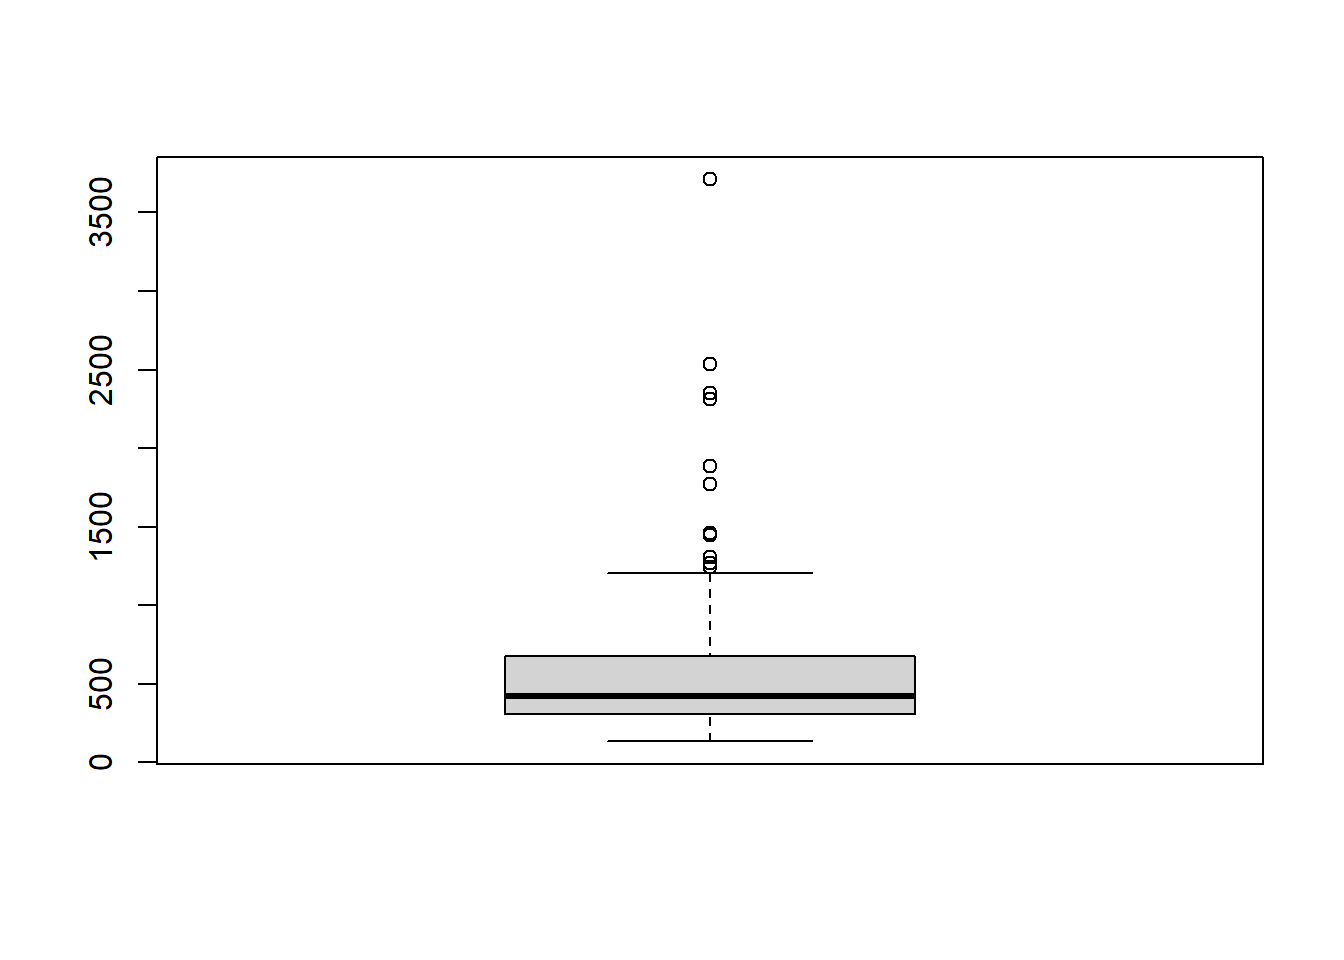
\includegraphics{Lab1_files/figure-latex/unnamed-chunk-8-1.pdf}

\hypertarget{section-11}{%
\subsection{12:}\label{section-11}}

\begin{Shaded}
\begin{Highlighting}[]
\NormalTok{a }\OtherTok{\textless{}{-}}\NormalTok{ feature\_1[}\DecValTok{6} \SpecialCharTok{:} \DecValTok{22}\NormalTok{]}
\NormalTok{a}
\end{Highlighting}
\end{Shaded}

\begin{verbatim}
##  [1] 55 56 57 58 59 60 61 62 63 64 65 66 67 68 69 70 71
\end{verbatim}

\hypertarget{section-12}{%
\subsection{13:}\label{section-12}}

\begin{Shaded}
\begin{Highlighting}[]
\NormalTok{b }\OtherTok{\textless{}{-}}\NormalTok{ feature\_1[}\FunctionTok{c}\NormalTok{(}\DecValTok{6}\NormalTok{, }\DecValTok{13}\NormalTok{, }\DecValTok{21}\NormalTok{, }\DecValTok{22}\NormalTok{, }\DecValTok{43}\NormalTok{)]}
\NormalTok{b}
\end{Highlighting}
\end{Shaded}

\begin{verbatim}
## [1] 55 62 70 71 92
\end{verbatim}

\hypertarget{section-13}{%
\subsection{14:}\label{section-13}}

\begin{Shaded}
\begin{Highlighting}[]
\NormalTok{c }\OtherTok{\textless{}{-}} \FunctionTok{c}\NormalTok{(a, b)}
\NormalTok{c}
\end{Highlighting}
\end{Shaded}

\begin{verbatim}
##  [1] 55 56 57 58 59 60 61 62 63 64 65 66 67 68 69 70 71 55 62 70 71 92
\end{verbatim}

\hypertarget{section-14}{%
\subsection{15:}\label{section-14}}

\begin{Shaded}
\begin{Highlighting}[]
\NormalTok{find\_a }\OtherTok{\textless{}{-}} \ControlFlowTok{function}\NormalTok{(str)\{}
  \FunctionTok{return}\NormalTok{ (}\FunctionTok{grepl}\NormalTok{(}\StringTok{"a"}\NormalTok{, str))}
\NormalTok{\}}

\NormalTok{str }\OtherTok{\textless{}{-}} \FunctionTok{c}\NormalTok{(}\StringTok{"joey"}\NormalTok{, }\StringTok{"phoebe"}\NormalTok{, }\StringTok{"monica"}\NormalTok{, }\StringTok{"chandler"}\NormalTok{, }\StringTok{"ross"}\NormalTok{, }\StringTok{"rachel"}\NormalTok{)}
\FunctionTok{sum}\NormalTok{(}\FunctionTok{as.integer}\NormalTok{(}\FunctionTok{lapply}\NormalTok{(str, find\_a)))}
\end{Highlighting}
\end{Shaded}

\begin{verbatim}
## [1] 3
\end{verbatim}

\hypertarget{d-factors}{%
\section{d) Factors}\label{d-factors}}

\hypertarget{section-15}{%
\subsection{16:}\label{section-15}}

Factor in R is \textbf{a variable used to categorize and store the data,
having a limited number of different values}.

Factors have limited number of different values, while vectors don't
have any limitation.

\begin{Shaded}
\begin{Highlighting}[]
\NormalTok{directions }\OtherTok{\textless{}{-}} \FunctionTok{c}\NormalTok{(}\StringTok{"West"}\NormalTok{, }\StringTok{"East"}\NormalTok{, }\StringTok{"East"}\NormalTok{, }\StringTok{"North"}\NormalTok{, }\StringTok{"West"}\NormalTok{, }\StringTok{"West"}\NormalTok{)}
\NormalTok{feature\_2 }\OtherTok{\textless{}{-}} \FunctionTok{factor}\NormalTok{ (directions)}
\end{Highlighting}
\end{Shaded}

\hypertarget{section-16}{%
\subsection{17:}\label{section-16}}

It isn't possible, because `South' isn't one of feature\_2's levels.

\hypertarget{section-17}{%
\subsection{18:}\label{section-17}}

\begin{Shaded}
\begin{Highlighting}[]
\FunctionTok{levels}\NormalTok{(feature\_2) }\OtherTok{\textless{}{-}} \FunctionTok{c}\NormalTok{(}\FunctionTok{levels}\NormalTok{(feature\_2), }\StringTok{"South"}\NormalTok{)}
\NormalTok{feature\_2}
\end{Highlighting}
\end{Shaded}

\begin{verbatim}
## [1] West  East  East  North West  West 
## Levels: East North West South
\end{verbatim}

\hypertarget{section-18}{%
\subsection{19:}\label{section-18}}

There is nothing important to report, everything works well.

\begin{Shaded}
\begin{Highlighting}[]
\NormalTok{feature\_2[}\DecValTok{1}\NormalTok{] }\OtherTok{\textless{}{-}} \StringTok{"South"}
\NormalTok{feature\_2}
\end{Highlighting}
\end{Shaded}

\begin{verbatim}
## [1] South East  East  North West  West 
## Levels: East North West South
\end{verbatim}

\hypertarget{e-missing-values}{%
\section{e) Missing values}\label{e-missing-values}}

\hypertarget{section-19}{%
\subsection{20:}\label{section-19}}

NA

\hypertarget{section-20}{%
\subsection{21:}\label{section-20}}

\begin{Shaded}
\begin{Highlighting}[]
\NormalTok{feature\_1[}\DecValTok{1}\NormalTok{] }\OtherTok{\textless{}{-}} \ConstantTok{NA}
\NormalTok{feature\_1}
\end{Highlighting}
\end{Shaded}

\begin{verbatim}
##   [1]  NA  51  52  53  54  55  56  57  58  59  60  61  62  63  64  65  66  67
##  [19]  68  69  70  71  72  73  74  75  76  77  78  79  80  81  82  83  84  85
##  [37]  86  87  88  89  90  91  92  93  94  95  96  97  98  99 100 101 102 103
##  [55] 104 105 106 107 108 109 110 111 112 113 114 115 116 117 118 119 120 121
##  [73] 122 123 124 125 126 127 128 129 130 131 132 133 134 135 136 137 138 139
##  [91] 140 141 142 143 144 145 146 147 148 149 150 151 152 153 154 155 156 157
## [109] 158 159 160 161 162 163 164 165 166 167 168 169 170 171 172 173 174 175
## [127] 176 177 178 179 180 181 182 183 184 185 186 187 188 189 190 191 192 193
## [145] 194 195 196 197 198 199 200 201 202 203 204 205 206 207 208 209 210 211
## [163] 212 213 214 215 216 217 218 219 220 221 222 223 224 225 226 227 228 229
## [181] 230 231 232 233 234 235 236 237 238 239 240 241 242 243 244 245 246 247
## [199] 248 249 250
\end{verbatim}

\hypertarget{section-21}{%
\subsection{22:}\label{section-21}}

mean() function can't calculate feature\_1's mean and returns NaN
because first element of this vector is missing.

We can set ``na.rm'' argument, true in mean() function to resolve this
problem.

\begin{Shaded}
\begin{Highlighting}[]
\FunctionTok{mean}\NormalTok{(feature\_1, }\AttributeTok{na.rm =}\NormalTok{ T)}
\end{Highlighting}
\end{Shaded}

\begin{verbatim}
## [1] 150.5
\end{verbatim}

\hypertarget{section-22}{%
\subsection{23:}\label{section-22}}

\begin{Shaded}
\begin{Highlighting}[]
\NormalTok{feature\_1[}\DecValTok{43}\NormalTok{] }\OtherTok{\textless{}{-}} \ConstantTok{NA}
\FunctionTok{which}\NormalTok{(}\FunctionTok{is.na}\NormalTok{(feature\_1))}
\end{Highlighting}
\end{Shaded}

\begin{verbatim}
## [1]  1 43
\end{verbatim}

\hypertarget{section-23}{%
\subsection{24:}\label{section-23}}

\textbf{NULL represents the null object in R}. NULL is used mainly to
represent the lists with zero length, and is often returned by
expressions and functions whose value is undefined.

\hypertarget{f-lists}{%
\section{f) Lists}\label{f-lists}}

\hypertarget{section-24}{%
\subsection{25:}\label{section-24}}

List is a list of variables which types could be different.

\hypertarget{section-25}{%
\subsection{26:}\label{section-25}}

list {[}x{]} will return a list which only contains the x\_th element of
list, while list {[}{[}x{]}{]} will return x\_th element of list, it
self.

\begin{Shaded}
\begin{Highlighting}[]
\NormalTok{lst }\OtherTok{\textless{}{-}} \FunctionTok{list}\NormalTok{(}\DecValTok{4}\NormalTok{, }\DecValTok{5}\NormalTok{, }\DecValTok{6}\NormalTok{, }\FunctionTok{list}\NormalTok{(}\DecValTok{7}\NormalTok{, }\DecValTok{8}\NormalTok{, }\StringTok{"xyz"}\NormalTok{))}
\end{Highlighting}
\end{Shaded}

\hypertarget{g-naming}{%
\section{g) Naming}\label{g-naming}}

\begin{Shaded}
\begin{Highlighting}[]
\NormalTok{named\_list }\OtherTok{\textless{}{-}} \FunctionTok{list}\NormalTok{(}\AttributeTok{a =} \DecValTok{1}\NormalTok{, }\AttributeTok{b =} \DecValTok{2}\NormalTok{, }\AttributeTok{c =} \DecValTok{3}\NormalTok{, }\AttributeTok{d =} \FunctionTok{c}\NormalTok{(}\DecValTok{4}\NormalTok{, }\DecValTok{5}\NormalTok{, }\DecValTok{6}\NormalTok{, }\DecValTok{7}\NormalTok{))}
\end{Highlighting}
\end{Shaded}

\hypertarget{section-26}{%
\subsection{27:}\label{section-26}}

First one returns a list contains 2, while other ones returns 2 itself.

it is a syntax sugar for {[}{[}{]}{]} because they both do the same
thing.

\begin{Shaded}
\begin{Highlighting}[]
\NormalTok{named\_list[}\StringTok{"b"}\NormalTok{]}
\end{Highlighting}
\end{Shaded}

\begin{verbatim}
## $b
## [1] 2
\end{verbatim}

\begin{Shaded}
\begin{Highlighting}[]
\NormalTok{named\_list[[}\StringTok{"b"}\NormalTok{]]}
\end{Highlighting}
\end{Shaded}

\begin{verbatim}
## [1] 2
\end{verbatim}

\begin{Shaded}
\begin{Highlighting}[]
\NormalTok{named\_list}\SpecialCharTok{$}\NormalTok{b}
\end{Highlighting}
\end{Shaded}

\begin{verbatim}
## [1] 2
\end{verbatim}

\hypertarget{h-data-frames}{%
\section{h) Data Frames}\label{h-data-frames}}

\hypertarget{section-27}{%
\subsection{28:}\label{section-27}}

\begin{Shaded}
\begin{Highlighting}[]
\FunctionTok{ncol}\NormalTok{(Orange)}
\end{Highlighting}
\end{Shaded}

\begin{verbatim}
## [1] 3
\end{verbatim}

\hypertarget{section-28}{%
\subsection{29:}\label{section-28}}

\begin{Shaded}
\begin{Highlighting}[]
\FunctionTok{nrow}\NormalTok{(Orange)}
\end{Highlighting}
\end{Shaded}

\begin{verbatim}
## [1] 35
\end{verbatim}

\hypertarget{section-29}{%
\subsection{30:}\label{section-29}}

\begin{Shaded}
\begin{Highlighting}[]
\NormalTok{f3 }\OtherTok{\textless{}{-}}\NormalTok{ Orange}\SpecialCharTok{$}\NormalTok{circumference}
\NormalTok{f3\_tmp }\OtherTok{\textless{}{-}}\NormalTok{ Orange[[}\DecValTok{3}\NormalTok{]]}
\end{Highlighting}
\end{Shaded}

\hypertarget{section-30}{%
\subsection{31:}\label{section-30}}

f3 is a vector.

Due to the dipersion of circumference feature, this data set had been
chosen randomly.

\begin{Shaded}
\begin{Highlighting}[]
\FunctionTok{table}\NormalTok{(f3)}
\end{Highlighting}
\end{Shaded}

\begin{verbatim}
## f3
##  30  32  33  49  51  58  62  69  75  81  87 108 111 112 115 120 125 139 140 142 
##   3   1   1   1   1   1   1   1   1   1   1   1   1   1   2   1   1   1   1   2 
## 145 156 167 172 174 177 179 203 209 214 
##   1   1   1   1   1   1   1   2   1   1
\end{verbatim}

\hypertarget{section-31}{%
\subsection{32:}\label{section-31}}

Tree feature is catagorical

\begin{Shaded}
\begin{Highlighting}[]
\FunctionTok{str}\NormalTok{(Orange)}
\end{Highlighting}
\end{Shaded}

\begin{verbatim}
## Classes 'nfnGroupedData', 'nfGroupedData', 'groupedData' and 'data.frame':   35 obs. of  3 variables:
##  $ Tree         : Ord.factor w/ 5 levels "3"<"1"<"5"<"2"<..: 2 2 2 2 2 2 2 4 4 4 ...
##  $ age          : num  118 484 664 1004 1231 ...
##  $ circumference: num  30 58 87 115 120 142 145 33 69 111 ...
##  - attr(*, "formula")=Class 'formula'  language circumference ~ age | Tree
##   .. ..- attr(*, ".Environment")=<environment: R_EmptyEnv> 
##  - attr(*, "labels")=List of 2
##   ..$ x: chr "Time since December 31, 1968"
##   ..$ y: chr "Trunk circumference"
##  - attr(*, "units")=List of 2
##   ..$ x: chr "(days)"
##   ..$ y: chr "(mm)"
\end{verbatim}

\hypertarget{section-32}{%
\subsection{33:}\label{section-32}}

\begin{Shaded}
\begin{Highlighting}[]
\NormalTok{s29 }\OtherTok{\textless{}{-}}\NormalTok{ Orange[}\DecValTok{29}\NormalTok{, ]}
\NormalTok{s29}
\end{Highlighting}
\end{Shaded}

\begin{verbatim}
##    Tree age circumference
## 29    5 118            30
\end{verbatim}

\hypertarget{section-33}{%
\subsection{34:}\label{section-33}}

It is a data frame with one row.

\hypertarget{section-34}{%
\subsection{35:}\label{section-34}}

\begin{Shaded}
\begin{Highlighting}[]
\NormalTok{Orange[}\FunctionTok{c}\NormalTok{(Orange}\SpecialCharTok{$}\NormalTok{Tree }\SpecialCharTok{==} \DecValTok{3}\NormalTok{), ]}
\end{Highlighting}
\end{Shaded}

\begin{verbatim}
##    Tree  age circumference
## 15    3  118            30
## 16    3  484            51
## 17    3  664            75
## 18    3 1004           108
## 19    3 1231           115
## 20    3 1372           139
## 21    3 1582           140
\end{verbatim}

\hypertarget{section-35}{%
\subsection{36:}\label{section-35}}

\begin{Shaded}
\begin{Highlighting}[]
\NormalTok{tmp }\OtherTok{\textless{}{-}}\NormalTok{ Orange[}\DecValTok{1} \SpecialCharTok{:} \DecValTok{10}\NormalTok{, }\FunctionTok{c}\NormalTok{(}\StringTok{"Tree"}\NormalTok{, }\StringTok{"age"}\NormalTok{)]}
\NormalTok{tmp}
\end{Highlighting}
\end{Shaded}

\begin{verbatim}
##    Tree  age
## 1     1  118
## 2     1  484
## 3     1  664
## 4     1 1004
## 5     1 1231
## 6     1 1372
## 7     1 1582
## 8     2  118
## 9     2  484
## 10    2  664
\end{verbatim}

\hypertarget{section-36}{%
\subsection{37:}\label{section-36}}

\begin{Shaded}
\begin{Highlighting}[]
\FunctionTok{median}\NormalTok{(Orange}\SpecialCharTok{$}\NormalTok{age)}
\end{Highlighting}
\end{Shaded}

\begin{verbatim}
## [1] 1004
\end{verbatim}

\hypertarget{i-export-and-import}{%
\section{i) Export and Import}\label{i-export-and-import}}

\hypertarget{section-37}{%
\subsection{38:}\label{section-37}}

\begin{Shaded}
\begin{Highlighting}[]
\NormalTok{df\_1 }\OtherTok{\textless{}{-}} \FunctionTok{tail}\NormalTok{(Orange, }\AttributeTok{n =} \DecValTok{15}\NormalTok{)}
\end{Highlighting}
\end{Shaded}

\hypertarget{section-38}{%
\subsection{39:}\label{section-38}}

\begin{Shaded}
\begin{Highlighting}[]
\FunctionTok{write.csv}\NormalTok{(df\_1, }\StringTok{"df\_1.csv"}\NormalTok{, }\AttributeTok{row.names =}\NormalTok{ F)}
\end{Highlighting}
\end{Shaded}

\hypertarget{section-39}{%
\subsection{40:}\label{section-39}}

\begin{Shaded}
\begin{Highlighting}[]
\NormalTok{df\_2 }\OtherTok{\textless{}{-}} \FunctionTok{read.csv}\NormalTok{(}\StringTok{"df\_1.csv"}\NormalTok{)}
\NormalTok{df\_2}
\end{Highlighting}
\end{Shaded}

\begin{verbatim}
##    Tree  age circumference
## 1     3 1582           140
## 2     4  118            32
## 3     4  484            62
## 4     4  664           112
## 5     4 1004           167
## 6     4 1231           179
## 7     4 1372           209
## 8     4 1582           214
## 9     5  118            30
## 10    5  484            49
## 11    5  664            81
## 12    5 1004           125
## 13    5 1231           142
## 14    5 1372           174
## 15    5 1582           177
\end{verbatim}

\end{document}
